\chapter{Literature review}

\label{chap:lit_rev}

In this chapter I provide an inventory of systems found in literature highlighting the opportunities that appear and are worth to be further investigated in this thesis. I will also describe and motivate the innovation introduced by RoomPlaces and how the system addresses and supports those opportunities.

Learning technologies groups all over the world are constantly working for improving systems that support teaching and learning inside school classrooms. In literature there are many examples on how the embodiment can improve the quality of interactive applications, among the advantages there is increase of students’ attention due to engagement and enjoyment in the topic of the lecture. Embodied design requires technical support that includes both hardware and software tools that are often built for a specific type of application and are not general enough for being reusable.

\section{Reusable indoor location framework}
The main contribution of this thesis is describing a first attempt of creating a reusable indoor location framework that is general enough to support the needs of applications in classrooms, based on the opportunities that can be found in literature. This type of applications has very specific requirements, first among all, the simplicity in setting up the system before the lesson. The vision for the future of this systems is that teachers themselves, without any special training, must be able to configure and use the applications. For this reason, only a lightweight infrastructure placement and an easy and fast configuration is acceptable for this scenario. All the overcomplicated details related to the low level technologies employed must be hidden to teachers and students and the only thing that matter is enable them to interact with the system in the most natural way possible.

Indoor location tracking is still an open problem in the research (Lymberopoulos et al. \cite{lymberopoulos:indoor_tracking}) and many teams are dealing with it. The purpose of this research is not researching a better solution to the problem, but evaluate existing technologies understanding their limits and obtaining a system that is precise and reliable enough for the purpose of tracking users and objects inside classrooms.

The main opportunity that can be deducted from the literature is the possibility of using the location as a driver for the simulation creating an interaction method. This interaction requires high reliability, but not necessarily a high precision. Depending on the application we can tolerate delays and reading errors. 

\subsection{Savannah project}
In Savannah project \cite{facer:savannah} is a participatory simulation where a group of ten children are playing the role of a pride of lions living in the Savannah. The main goal of the game is understand and survive in this territory. For doing so they are required to develop strategies for balancing a series of activities like running, sleeping, drinking and attacking preys. To add realism and improve engagement the game is conducted in an outside field, every child has a PDA connected using Wi-Fi with a server that runs the simulation. Every action (sounds played, prays that can be killed, water sources, etc.) is location dependent. The tracking system employed is GPS that is actually the better choice in outdoor applications. This tracking system is very straightforward to implement since the output are geographical coordinates, however it provides low level information that must be elaborated before it can be used in this application. The needed information is the location of the user, for example: near a pray, in an hot area or in the water. Another very important feature is the ability of receiving a stream of events and based on it decide the available interactions. Instead of having coordinates that have to be continuously compared with the coordinates of every other entity in the game, the only needed information is the proximity of a children (a lion) and a prey or the duration of the stay in a pre-defined area (easy computable because it is the time between arrival and departure events on that area). Using this framework, the system implementation could be reduced to a list of behaviors assignable to objects proximity events, for example playing a sound near a prey or adding points while in the water.

\subsection{Ambient Wood}
Ambient Wood \cite{randell:ambient_wood} is a playful learning experience based on a field trip in English woodlands. Each child has a PDA connected with a set of hardware devices used to interact with the virtual environment and also with a Den, where a facilitator guides them in the exploration of the environment. The goal of the game is explore, consolidate, hypothese, experiment and reflect about various aspects of plants and animals living in the different habitats in the wood during a visit that lasts around one hour. In this projects are used radio frequency beacons in order to detect the proximity of an area of interest. As already pointed out in Savannah project the system needs a service that alerts the PDAs when it is inside a certain area, in this case for playing a sound or initiate some other interaction. This system employs an ad-hoc wireless technology developed starting from low level hardware components like PIC microcontrollers, FM transmitter and receiver modules. This approach, despite interesting, is challenging and time consuming because the system requires to be designed starting from the electrical circuits and only after a long period of time it can be considered reliable enough for being used for this applications. The location beacons emit one packet per second and the probability of being received, according to the authors, is around 95\% if the transmitter is in a 10 meters’ radius of the receiver. An opportunity that emerge from this scenario is the possibility for the facilitator (in the Dan) of knowing real-time the location of children for safety purposes or for checking if they're executing the assignment or not.

\subsection{Environmental Detective}
Environmental Detective \cite{klopfer:environmental_detectives} is a participatory simulation where students divided in groups participate in a real-time simulation of an environmental disaster where the watershed of a small city has been polluted by an industrial plant. The goal of the simulation is discovering what is the plant (or the plants) where the pollution is coming from, how the pollution enters the water stream and how to mitigate the effect. In order to interact with the real world, the simulation uses the GPS and a custom sets of virtual maps that indicates where the child is in the simulated village. This scenario provides an interesting new opportunity based on the possibility of (simulating) drilling a water sample extraction in every point and receiving a response from the system that depends from the position of the mobile device. This situation requires the position (not only an object proximity), but it is not required an high precision, for example it is easy to divide the area and associate certain sampling values to every one of them.

\subsection{RoomQuake}
RoomQuake \cite{moher:roomquake} is an Embedded Phenomena \cite{moher:embedded} where seismological events are simulated inside the classroom with the goal of allowing students to learn the skill of locating the epicenter and understanding the meaning of earthquake magnitude. Virtual seismographs are places in fixed positions of the classroom and they display seismic waves intensity in that point of the room. Students are required to use information from the simulated instruments and apply the mathematical trilateration technique in order to locate the epicenter. This application highlights the need of having both real and virtual resources embedded in the classroom physical space. Earthquakes can be represented as virtual resources with associated the position of their epicenter and the magnitude (that must be stored as extra parameter). Seismometers are real resources because they are computers or tablets that have a fixed position in the room. The positions of both virtual and physical resources are needed in order to calculate the distance from the epicenter that is directly proportional to the intensity of the displayed waves.


\section{Duality tracking system}
A second contribution of this thesis is demonstrating how to create a flexible tracking system that has the ability to track both moving objects (containing beacons, \ref{fig:use_case_1}) and users carrying mobile devices (\ref{fig:use_case_2}). The two modality are dual and the problem is completely symmetric, since in the first one the mobile devices have fixed locations and objects are free to move around and in the second happens the exact opposite where beacons are in fixed and predetermined locations and used for tracking the location of mobile devices. The proposed solution also supports a hybrid between the two: a system that can track both objects and users at the same time (\ref{fig:use_case_3}).

\begin{figure}
\centering
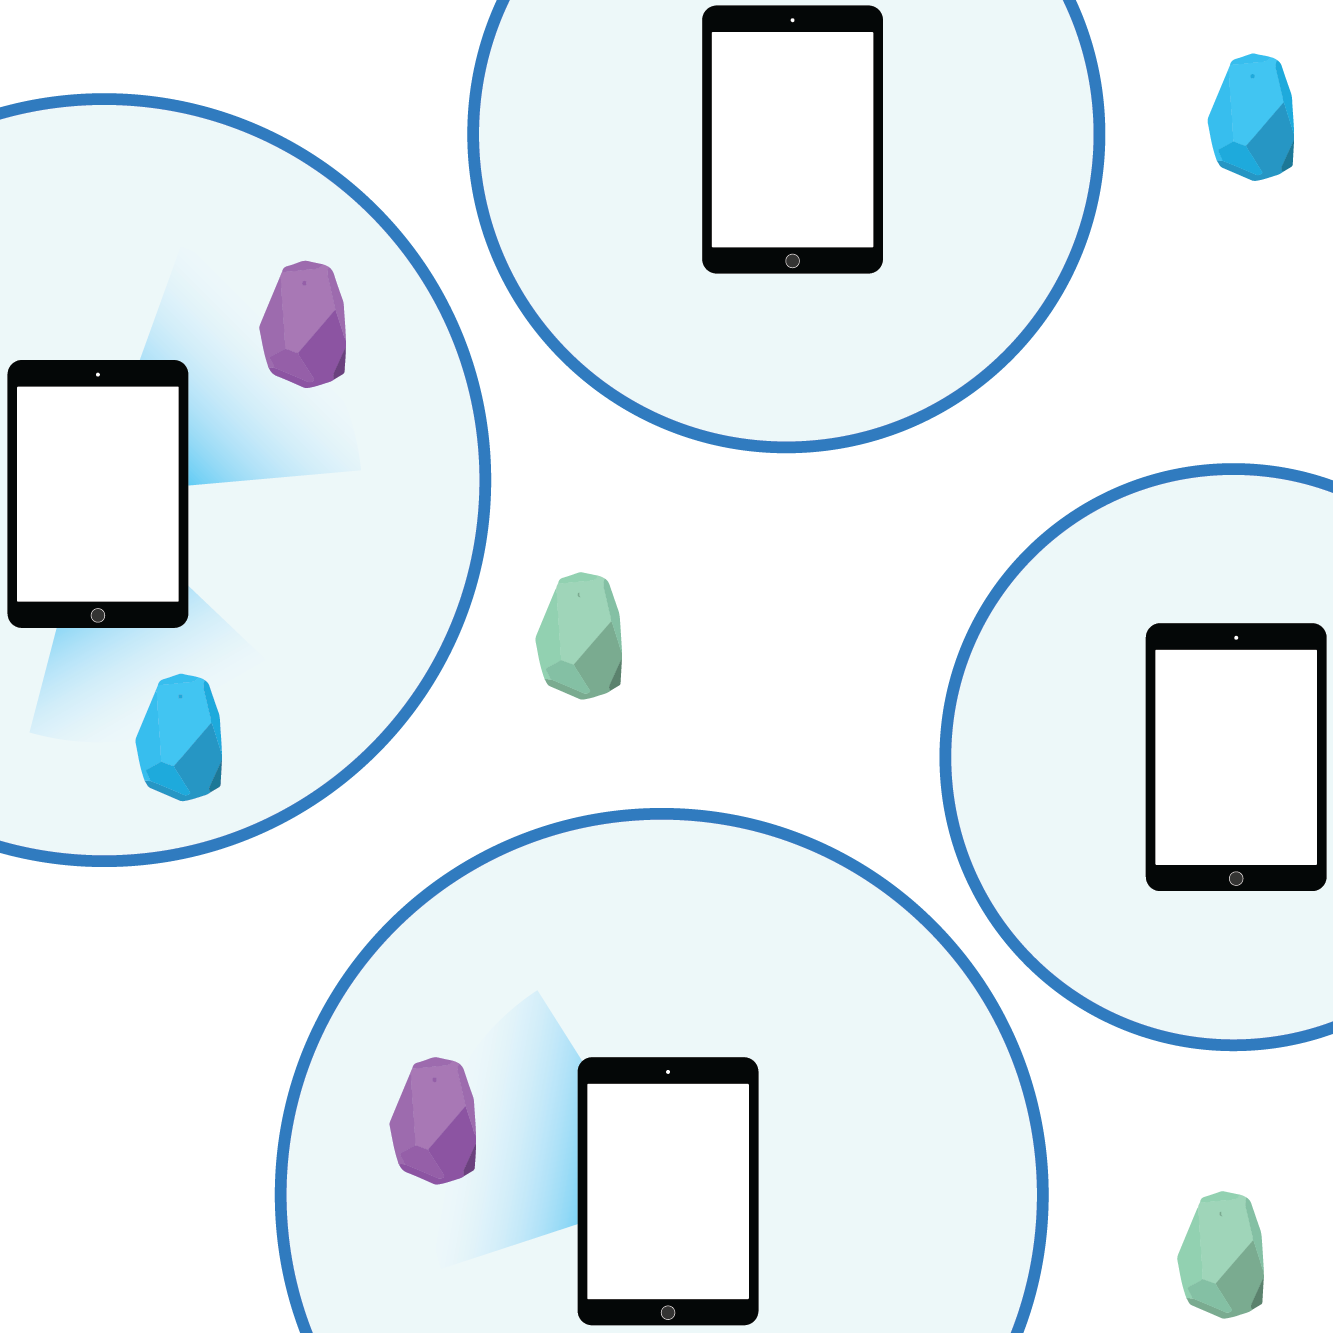
\includegraphics[width=2.5in]{images/room-places-use-case-1.png}
\caption{tablets tracking moving beacons}
\label{fig:use_case_1}
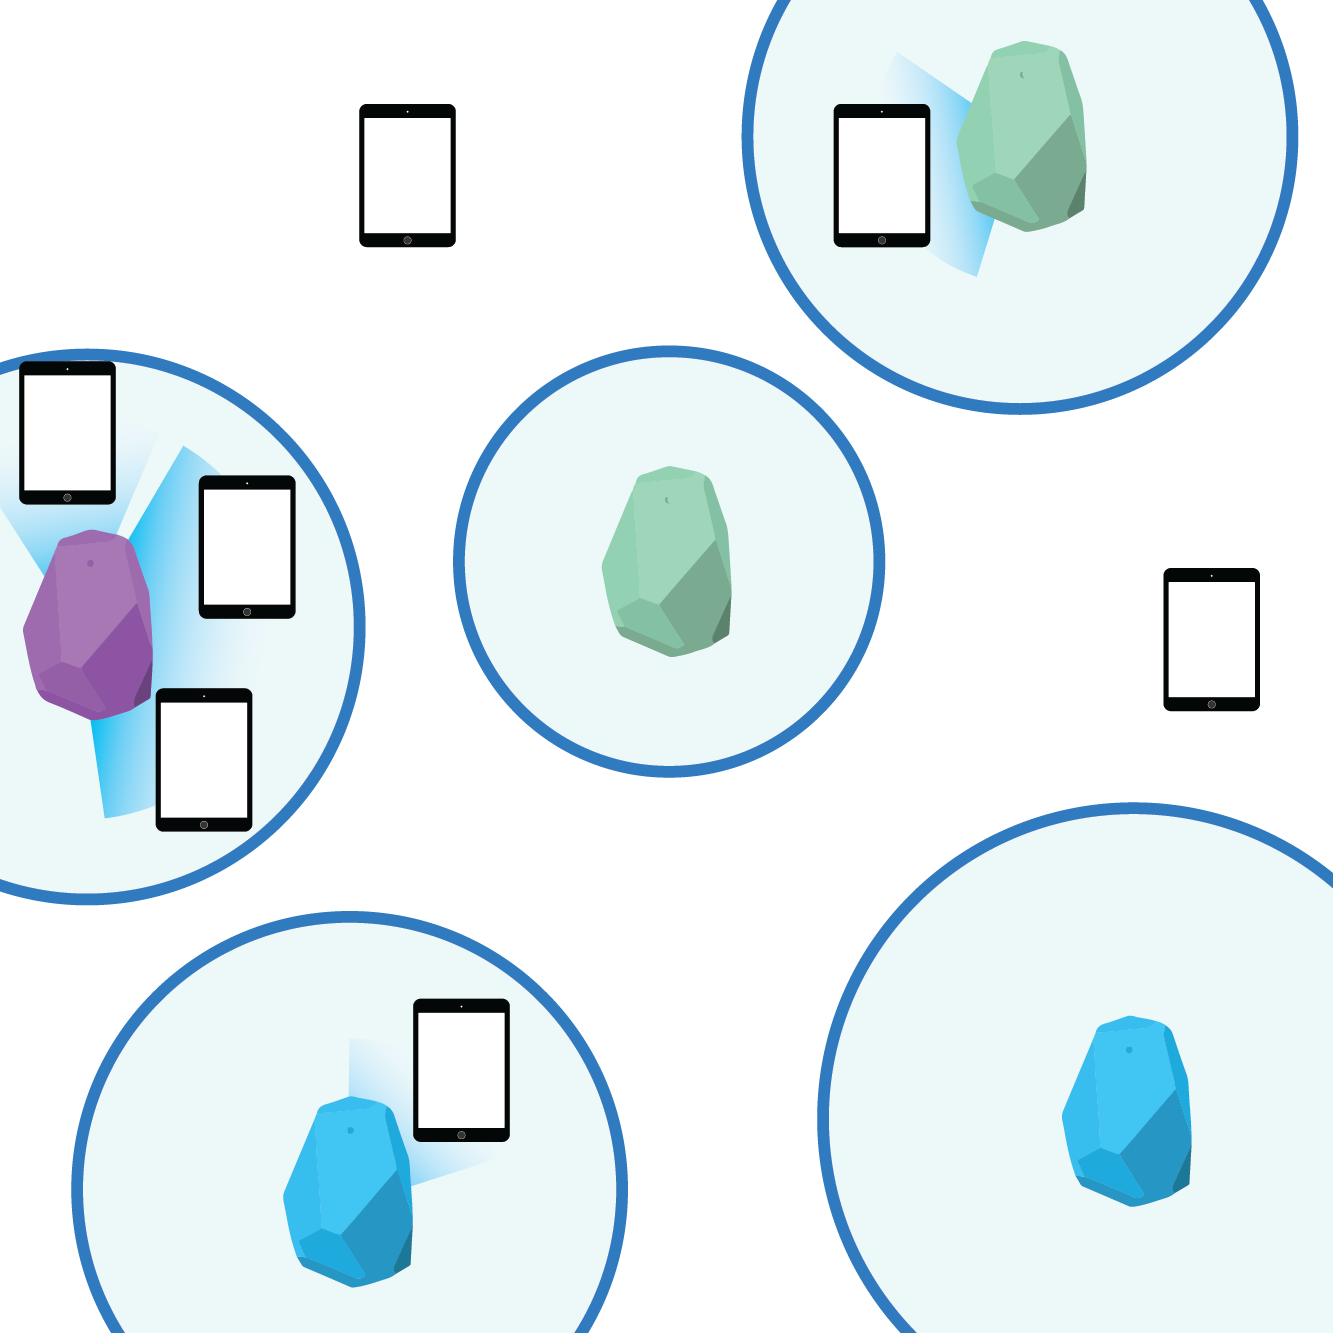
\includegraphics[width=2.5in]{images/room-places-use-case-2.png}
\caption{beacons tracking moving tablets}
\label{fig:use_case_2}
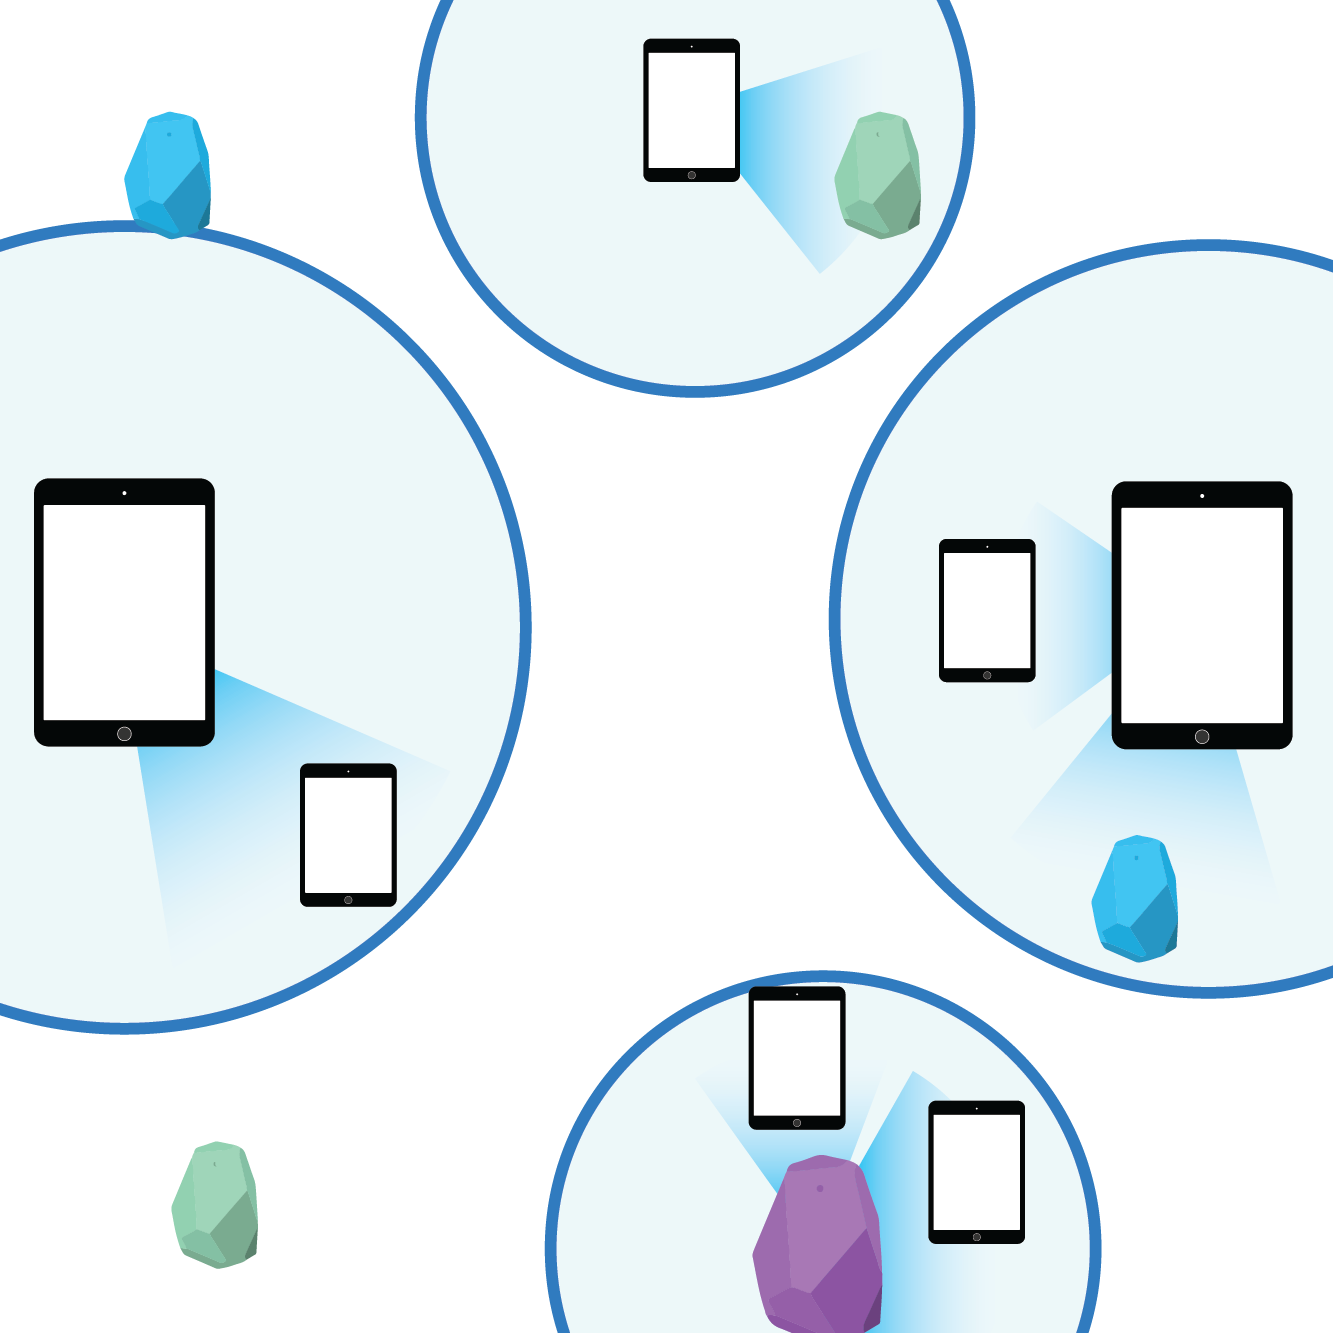
\includegraphics[width=2.5in]{images/room-places-use-case-3.png}
\caption{tablets and beacons tracking every Bluetooth LE device}
\label{fig:use_case_3}
\end{figure}

The first analyzed model and starting point for the discussion is the Apple iBeacon. It was created in order to deliver personalized content directly to the user smartphone when it is in proximity of a specific point. This technology is well suited for stores because it enables to target specific users with discount and promotions when they are near a specific product. In order to achieve this goal, a set of beacons is placed around the store, every one of them has a different code that transmits at fixed time interval on a certain radio frequency using Bluetooth LE protocol. Enabled mobile phones, when the store application is installed, are able to detect the beacon and they recognize it using its unique code and react providing personalized content to the user. An example on how, conceptually, this model was already applied inside learning sciences is Savannah project \cite{facer:savannah}, where mobiles were tracked (using GPS) used a fixed radio emitting infrastructure (the constellation of GPS satellites). 

The beacon model enables a new set of interactions that are based on the actual location of the user and it is ubiquitous for the characteristic of requiring very simple external hardware (iBeacons) and very low power that doesn't affect the duration of the battery of mobiles. Also the maintenance of beacons is very cheap since they can remain active for years with a small battery. This thesis proposes an improvement that can be obtained changing the assumption that the beacon must be the fixed object in the room and mobiles must change position. There are opportunities that are enabled using mobiles for tracking beacon positions. An important opportunity is the usage of location dependent collaboration resources: tangible objects containing beacons shared by many users that are associated with a possible interaction with the system. The interaction can depend from who is carrying the resource and from where the user (or an object) is in a precise moment.

In the following sub-sections, I report different systems that are already tracking radio beacons using a static positioned receiver and speculate about how much can be interesting adding flexibility to this models.

\subsection{Huting of the Snark}
In the Hunting of the Snark \cite{price:snark}, students investigate and discover characteristics of a virtual imaginary creature (called the Snark) hidden within the virtual space, co-located with the physical space of the classroom. Students use a number of physically-digitally coupled tools to locate and interact with the imaginary and elusive creature while it moves across "land, air and water" \cite{price:snark}. Technologies are employed in order to provide ways for interacting with the creature. An ultrasound based indoor tracking system is used in order to locate the PDAs used by children and provides an output dependent from their location. Another interaction happens using physical tokens that have to be placed at the entrance of a cave, and depending on the token used students can hear different "atmosphere" noises from inside the cave. In this context, two different ad-hoc systems were used, but there is the opportunity to unify them making easier to develop applications that use both.

\subsection{AquaRoom}
In AquaRoom \cite{novellis:acqua_room} students take the role of hydro geologists with the task of mapping a subterranean aquifer system (mapped to their classroom floor plan). Using this information they have to decide where to locate a new chemical plant within the local community to minimize potential environmental impacts. In order to accomplish this task, students "inject tracer dyes" and obtain water samples using a portable tablet-based "drilling unit". A suction cup attached to a (non-functional) cable is used to select locations for dye injection or water sampling. Test tubes capped with I-Buttons serve as simulated dye sources and sample repositories. Students "inject" dyes by inserting the test tubes into USB readers attached to the tablet drilling unit, with the liquids virtually running through the cabling. The interactive interface on the tablets allows them to manually mark the injection location, based on a grid system defined by the tiles on the room’s drop ceiling. Water samples are subsequently collected in a similar fashion, and tested for the presence of dyes using a simulated spectrometer represented by a shared desktop computer with its own USB reader. The injection of a dye followed by sampling allows students to establish the presence of an aquifer and the direction and rate of flow, which are marked on the tablet map and on a collective classroom map. This scenario highlights the need of a system that reliable recognizes under which tile the user is located without requiring a manual input. Since the position is discrete it could be easy to place fixed beacons near the tiles and associate the user position with the nearest beacon.

There is also another opportunity that emerges from this study: tracing the individual paths of the children while they're exploring the "subsoil" of their classroom. Since the position is self reported, can we trust it? Is it possible to combine user input with a tracking system prediction?

\section{Memory associated with physical objects}
The third contribution is describing and analyzing a technique for embedding information inside physical objects creating the concept of \textit{artifact as containers} or \textit{tangible containers}. The goal of the implementation explained in this thesis is not supporting every kind of data structure needed by applications, but is building a simple system complete enough for supporting the majority of the applications built in the past and creates the foundations for building more complex systems.

This contribution is driven by the need of creating a reusable system keeping track of virtual state of objects that can be combined with their location for creating new way of interacting with digital worlds. The opportunity to augment the reality with the information contained in tangibles: displaying personalized content on wall mounted screens or use every object as an authentication key for enabling hidden functionalities are only some of the new opportunities that are made possible with that capability.

Associating information with objects is not something new in Human Computer Interaction, actually it is done in every application development, but every time in a different and custom way depending from the features that are needed. Usually this is a task done in the back-end that has to be queried introducing latency and degrading user experience. I want to demonstrate that is possible to implement it in a distributed software scenario and is possible to introduce a hidden synchronization mechanism for separate the notion of data inside an object from the technology used for storing that data. In the next subsections I report different systems and I describe how they implement this capability in order to highlight the opportunity of simplifying the development process and include this capability in a framework.

\subsection{Hunger Games}
Hunger Games \cite{gnoli:hunger_games} is a participatory simulation designed to allow upper elementary school learners to explore fundamental concepts of competitive and cooperative games in the context of animal foraging. In Hunger Games the authors transform the physical space of the classroom into a natural habitat containing six food patches of different richness. Each student in the classroom receives a stuffed animal with an RFID tag embodied in it, which acts as his or her avatar during the activity. Whenever a student walks to a patch and places their avatar on top of it, the RFID reader embedded in the patch recognizes the tag and starts to provide energy to the student's avatar at a rate dependent on patch quality and competition (i.e. how many avatars are feeding off the same patch at the same time). After the activity students observe and reflect on their individual and collective foraging patters and design new strategies to improve their individual and/or collective outcome. In this scenario the tracking system made with RFID readers is completely separate with the system that store the energy levels of the avatars and that contains the parameters of the patches.

\subsection{BeeSim}
BeeSim \cite{peppler:beesim} is a participatory simulation which puts young children in the shoes of honeybees collecting nectar. The simulation makes extensive use of wearable technologies and aims at teaching kids about both the value of communicating nectar sources to other bees and the difficulty of finding nectar. Students assume the role of a honeybee looking for nectar by wearing a "ForagerBee" glove (a sensor embedded wearable made with LilyPad Arduino platform). Kids have only 45 seconds to collect as much nectar as possible (nectar level indicated with a led bar) while wrestling with the constraints of the system (e.g. limited nectar carrying capacity). Children take turns hunting for nectar. As the glove exchange happens, the child returning from the hunt can try to communicate the location of high-yield flowers to the “next bee”, through the use of nonverbal language. Once each child had their chance to wear the glove and hunt for nectar, the team with the most nectar is the “most prepared for winter” and therefore the winning team.

In order to collect nectar, the "ForagerBee” glove has a sensor that reads voltage over a resistor. Every flower (and the bee hive) has a different resistor that leads to a different voltage value reading. In order to store the amount of nectar collected, every glove is connected (using XBee wireless technology) to a central computer, that memorizes the amount of nectar collected and waits for the child to go to the bee hive for dropping it off. In this system, the proximity tracking  (made with a resistor and a voltage level sensor) and the nectar collected levels memory are kept separated introducing a series of challenges for the developers. They need a different resistor for every one of them making more difficult the initial setup because the voltage level must be measured for every flower. The substitution of broken resistors requires a physically identical resistor. 

\subsection{Virus Simulation}
Virus simulation by Colella \cite{colella:virus} is a \textit{participatory simulation} where students wore small portable computers called "Thinking Tags" around their necks with LED displays showing how many people every single individual had met during the activity and whether or not they are infected with the virus. The thinking tags are infrared receivers and transmitters that give the students the ability to transfer the virus to others by walking up to them. The goal of the activity was teaching to the students how to infer the rules that govern the simulation (e.g., virus latency, degree of contagiousness, who was the first infected agent, etc.). In this system the state of the objects is physically memorized inside the "Thinking Tags", since they are small computers, they have their own memory. This approach is successful in the scenarios where the information contained is changed only for the object itself and doesn't have to be accessed from remote objects (is not possible to know if an individual is infected or not until a teacher have physical access to the \textit{Thinking Tag}).

\section{High Level Application Programming Interface}
A very important feature, that allows all the three previously presented contributions to became a reality and the system to collaborate with external environments, is the presence of an high level set of APIs (Application Programming Interfaces). This feature is important in order to provide an easy and user friendly access to all the capabilities of the system. A technical description on how this APIs are implemented is present in the  \autoref{apdx:roomplaces_api}, in this section I explain what are the advantages and the motivations that drove the development of them.

The first motivation is related to the capability of the system of being ready to be used out of the shelf. During the development of scientific investigations for educational purposes the developer must spend the time implementing the application functionalities, not carrying about the technical details of the underlying technologies, in other words: I cannot expect a deep knowledge from the developer on how the system works. Reliable \textit{tracking system} and \textit{tangible containers} became a reality thanks to a huge amount of code (running on different machines) that manages the synchronization of all the components behind the scenes. Thanks to this APIs developers are allowed to use the tracking capabilities and tangible containers as services that can be used inside their environments and with their favorite programming language. The APIs are provided as simple native libraries (I implemented them in JavaScript, Swift and Ruby). 

An important point that I want to highlight and second motivation for using native APIs is that all the information is safely stored on a central server and the APIs are a simplified way for accessing and modifying this information. In case a component of the developed system crashes it is always possible to restore the state after the crash because all the objects provided by the APIs are synchronized behind the scenes. It is also important to safely store the data for research purposes: after the application stops when its time to analyze the data they can be found on the server, there's no need to use an external system for retrieving them from all the computers that run the application.

The third motivation for providing the needed information as a service is the possibility to integrate it in already existing systems. This is especially important for learning applications that are almost always developed iteratively and in which the functions are implemented in different moments. The user study in \autoref{chap:user_study} is an example in which the tracking system was used only in the last phase of the study and its integration did not require extra effort from the developer perspective. Integrating a tracking system inside pre-existing systems can enable new possibilities, for example is possible to create a distributed logging system that can track actions of the users (and safely store them on the central server) and report in real-time the behavior of the class to the teacher. Another opportunity is improving the security of the classrooms and compliance insurance: notify teachers or parents when children live the school if not previously authorized.
